\documentclass{article}
\usepackage{ctex}
\usepackage[a4paper, left=2.5cm, right=2.5cm, top=2.54cm, bottom=2.54cm]{geometry}
\usepackage{graphicx}
\usepackage{caption}
\usepackage{subcaption}
\usepackage{multirow}
\usepackage{multicol}
\usepackage{booktabs}
\usepackage[normalem]{ulem}
\usepackage{eqparbox}
\usepackage{listings}
\usepackage{mdframed}
\usepackage{amsmath}
\usepackage{enumerate}
\usepackage{placeins}
\usepackage{float}
\usepackage[dvipsnames]{xcolor}  % 使用 xcolor 包的 dvipsnames 选项
\usepackage[table,xcdraw]{xcolor}
% \usepackage{minted}
\useunder{\uline}{\ul}{}
\definecolor{code_bgc}{RGB}{255, 253, 253}  % 定义一个非常淡的粉色
\lstset{
    numbers=left,                   % 在左侧显示行号
    numberstyle=\color{Lavender},  % 设置行号的样式
    % frame=single,                   % 添加框架
    rulecolor=\color{black},        % 设置框架的颜色
    tabsize=2,                      % 设置tab的宽度
    breaklines=true,                % 自动折行
    breakatwhitespace=false,        % 在空白处折行
    escapeinside={\%*}{*)},         % 如果你想在代码中添加LaTeX代码,可以在此处设置
    keywordstyle=\color{RedViolet},      % 设置关键字的颜色
    commentstyle=\color{Salmon},   % 设置注释的颜色
    stringstyle=\color{RoyalBlue},      % 设置字符串的颜色
    basicstyle=\footnotesize,       % 设置代码的字体大小
    columns=fullflexible, 
    xleftmargin=2em,                % 设置左边距
    backgroundcolor=\color{code_bgc}, % 设置背景颜色
}
\newenvironment{codedisplay}[2]
{
    \begin{multicols}{3}
        \lstinputlisting[language={#1}]{#2}
    \end{multicols}
    
}

\begin{document}

\begin{table}
    \begin{tabular}{clllll}
    \multicolumn{4}{c}{\multirow{3}{*}{
\includegraphics[width=4.5cm]{assets/image.png}
    \fontsize{30}{35}\selectfont\kaishu 实验报告}}            & \quad 专业: & {\ul{\eqparbox{col4}{\quad 电子信息工程 \quad}}}     \\
    \multicolumn{4}{c}{}                                      & \quad 姓名: & {\ul {\eqparbox{col4}{\qquad 冯静怡}}}        \\
    \multicolumn{4}{c}{}                                      & \quad 学号: & {\ul {\eqparbox{col4}{\quad 3220104119}}} \\
    课程名称: & {\ul {\eqparbox{col1}{\quad 微机原理及应用实验\quad}}} & \quad 指导老师:    & {\ul {\eqparbox{col2}{胡斯登\quad}}} 
     & \quad 地点: & {\ul {\eqparbox{col4}{ 紫金港东三406}}}   \\
    实验名称: & {\ul {\eqparbox{col1}{\quad FFT\quad }}}       &\quad 同组学生: & {\ul {\eqparbox{col2}{陈亦乔\quad} }}
    &\quad 日期: & {\ul {\eqparbox{col4}{\today}}}      
    \end{tabular}
    \end{table}

\section{实验目的}
\begin{enumerate}
    \item 掌握单片机AD采样的使用方法(DMA);
    \item 掌握单片机FFT的使用方法。
\end{enumerate}
\section{实验原理与思路}
\subsection{ADC(Analog to Digital Converter)}
\paragraph{原理:}
ADC(模数转换器)的作用是将连续的模拟信号转换为离散的数字信号。STM32中的ADC模块通常具有以下特性:
\begin{itemize}
    \item 分辨率:12位分辨率,可以产生0到4095之间的数字值。
    \item 采样率:指每秒钟ADC可以进行多少次转换,本实验通过设置TIM3,通过TIM3计时器溢出从而调用ADC。
    \item 通道:设置GPIO口进行AD转换。
    \item 转换模式:包括单次转换、连续转换和扫描模式,本实验采用单次转换。
\end{itemize}
\begin{figure}[H]
    \centering
    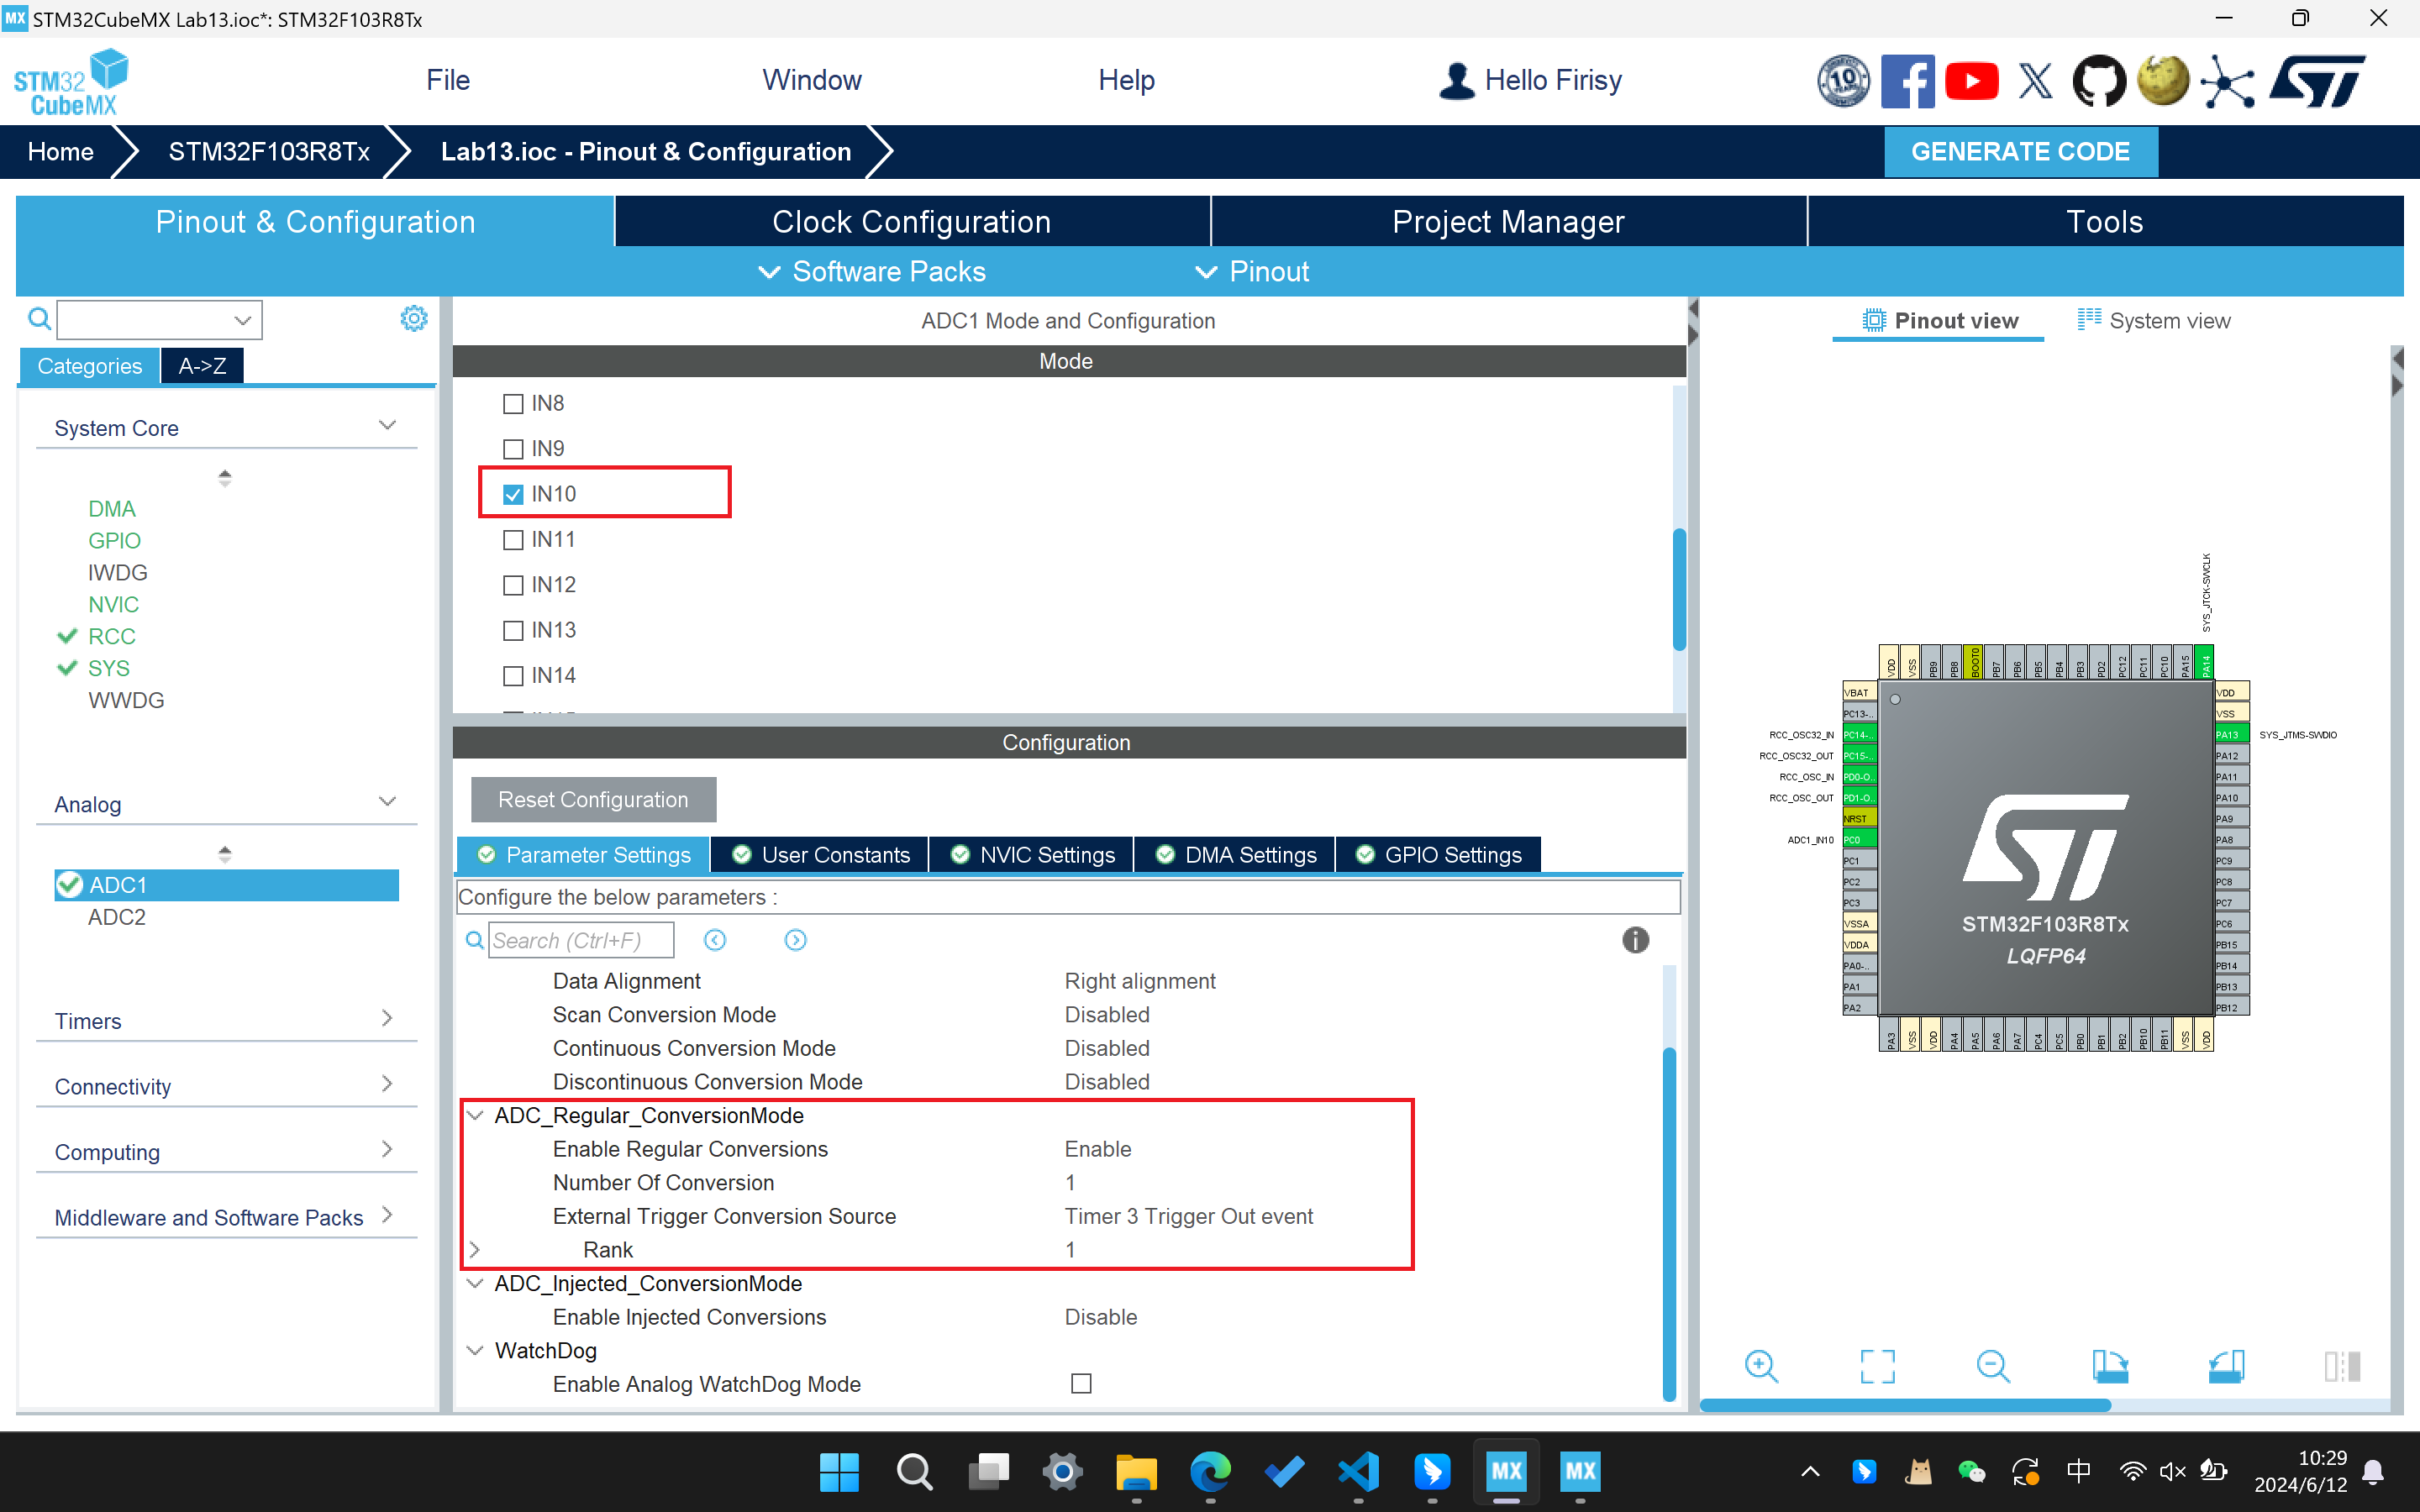
\includegraphics[width=0.8\textwidth]{assets/3.png}
    \caption{AD转换设置}
\end{figure}
\paragraph{工作流程:}
\begin{itemize}
    \item 设置ADC参数,包括分辨率、采样时间、通道等。
    \item 启动ADC进行采样。
    \item 将采样得到的模拟信号转换为数字信号。
\end{itemize}
\subsection{DMA(Direct Memory Access)}
\paragraph{原理:}
DMA(直接内存访问)模块允许外设(如ADC)在不经过CPU的情况下,直接将数据传输到内存或从内存传输到外设,从而提高数据传输效率,减轻CPU负担。
\begin{figure}[H]
    \centering
    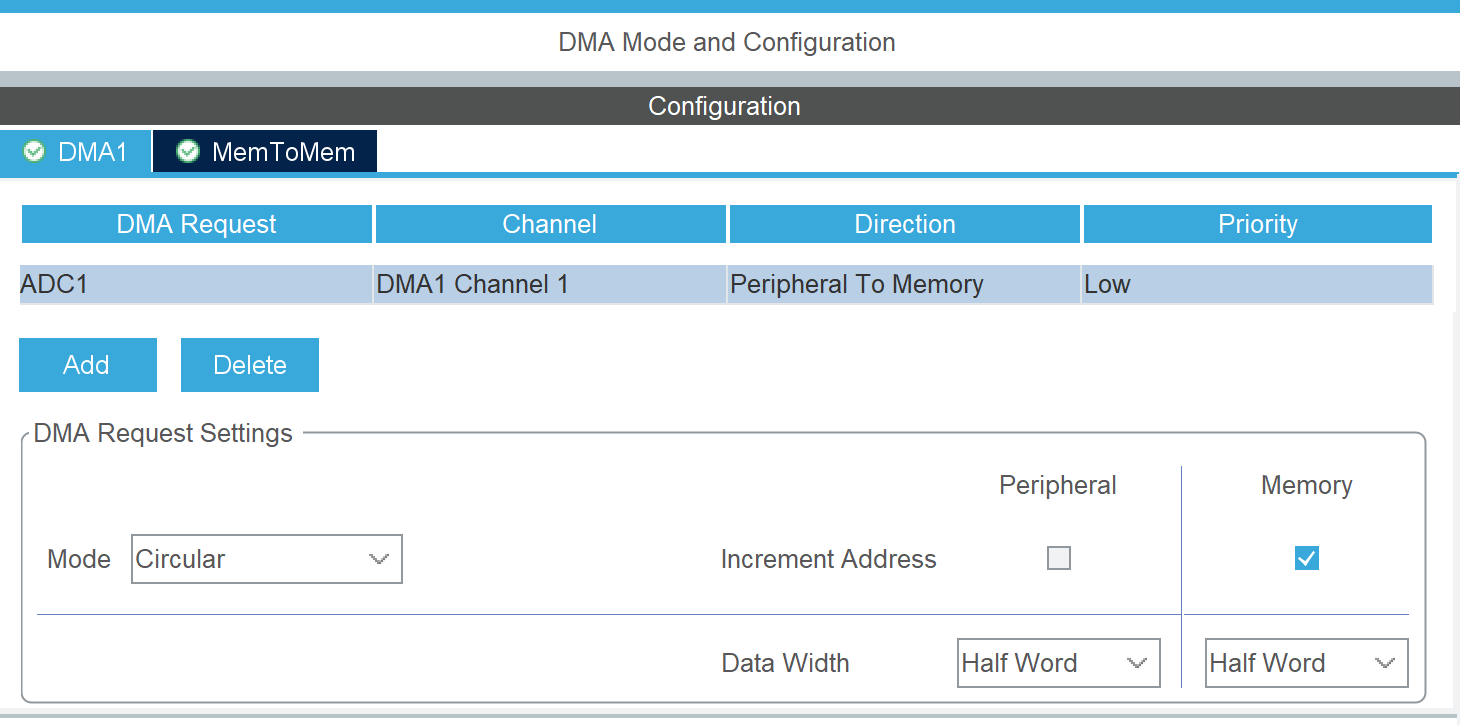
\includegraphics[width=0.8\textwidth]{assets/4.png}
    \caption{DMA传输}
\end{figure}
\paragraph{工作流程:}
\begin{itemize}
    \item 配置DMA传输方向(如从外设到内存),模式为循环,数据长度为半字即16位。
    \item 设置DMA的源地址和目标地址。
    \item 启动DMA,使其在ADC完成数据转换后自动将数据传输到内存。
\end{itemize}
\subsection{ADC与DMA结合}
\begin{enumerate}
    \item 初始化设置ADC和DMA。
\begin{lstlisting}[language={C}]
HAL_ADCEx_Calibration_Start(&hadc1);    //校准ADC,通过校准可以减少ADC转换中的误差。
HAL_ADC_Start_DMA(&hadc1,(uint32_t *)sampleData,FFT_NUM);   //启动ADC,并使能DMA传输,将采样数据传输到内存中(sampleData)。
HAL_TIM_Base_Start(&htim3); //启动TIM3计时器,通过TIM3计时器溢出来触发ADC采样。
\end{lstlisting}
    \item 设置ADC-DMA采样完成中断回调函数,当ADC采样完成时,停止TIM3计时器,停止ADC采样,并设置采样完成标志位。
\begin{lstlisting}[language={C}]
void HAL_ADC_ConvCpltCallback(ADC_HandleTypeDef *hadc)
{
    if(hadc == &hadc1)  //ADC转换中断
    {
        HAL_TIM_Base_Stop(&htim3);  //停止TIM3计时器
        HAL_ADC_Stop_DMA(&hadc1);   //停止ADC-DMA
        isSampleReady = 1;          //标志位置1
    }
}
\end{lstlisting}
    \item 在主函数中,当采样完成标志位为1时,进行数据处理。
\begin{lstlisting}[language={C}]
if(isSampleReady == 1) // 标志位置1
{
    dataIn[i] = sampleData[i]*3.3/4096; //处理输入数据转换为正确的浮点型
    /* 数据处理过程略 */
    isSampleReady = 0;  //标志位清零
    HAL_ADC_Start_DMA(&hadc1,(uint32_t *)sampleData,FFT_NUM);//开始新一轮数据的读入
}
\end{lstlisting}
\end{enumerate}
\subsection{FFT(Fast Fourier Transform)}
\paragraph{原理:}
FFT(快速傅里叶变换)是一种用于计算离散傅里叶变换(DFT)的高效算法。它将时域信号转换为频域信号,以分析信号的频率成分。
\begin{lstlisting}{language=c}
#include "arm_math.h"
#include "arm_const_structs.h"
\end{lstlisting}
使用以上两个ARM自带的数学库,执行FFT操作:
\begin{lstlisting}[language=c]
for(i=0;i<FFT_NUM;i++)
{
    fftIn[2*i] = sampleData[i]*3.3/4096;    //处理输入数据,数组[2*i]为实数部分,数组[2*i+1]为虚数部分
    fftIn[2*i+1] = 0 ;
}
arm_cfft_f32(&arm_cfft_sR_f32_len256,fftIn,0,1);    //库函数进行FFT
for(i=0;i<FFT_NUM;i++)
{
    sampleDataFreMag[i] = sqrtf(fftIn[2*i]*fftIn[2*i]+fftIn[2*i+1]*fftIn[2*i+1])/FFT_NUM;   //将FFT结果转换为可读性的幅值结果
}
\end{lstlisting}
其中$\texttt{arm\_cfft\_f32()}$各个参数含义:
\begin{lstlisting}{language=c}
/*
* @details
* @brief       Processing function for the floating-point complex FFT.
* @param[in]      *S    points to an instance of the floating-point CFFT structure.
* @param[in, out] *p1   points to the complex data buffer of size <code>2*fftLen</code>. Processing occurs in-place.
* @param[in]     ifftFlag       flag that selects forward (ifftFlag=0) or inverse (ifftFlag=1) transform.
* @param[in]     bitReverseFlag flag that enables (bitReverseFlag=1) or disables (bitReverseFlag=0) bit reversal of output.
* @return none.
*/
\end{lstlisting}
\section{实验结果}
设置输入频率为40kHz,1.65V直流偏置,1.65V的幅值,并将$\texttt{sampleDataFreMag}$ add to watch,得到以下两个数据显著不为0.
\begin{figure}[H]
    \begin{subfigure}{0.5\textwidth}
        \centering
        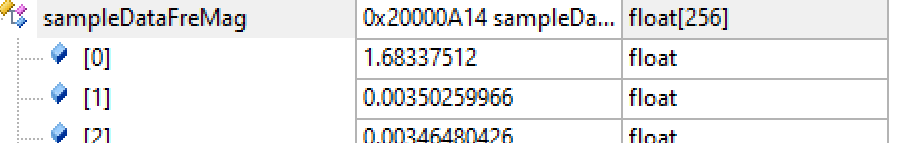
\includegraphics[width=0.8\textwidth]{assets/1.png}
        \caption{$\texttt{sampleDataFreMag[0]}$}
    \end{subfigure}
    \begin{subfigure}{0.5\textwidth}
        \centering
        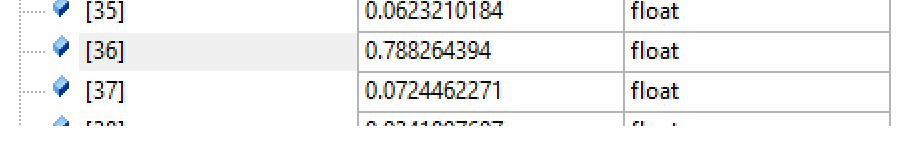
\includegraphics[width=0.8\textwidth]{assets/2.png}
        \caption{$\texttt{sampleDataFreMag[36]}$}
    \end{subfigure}
    \caption{实验结果}
\end{figure}
通过计算可以得到:\newline
TIM3的ARR设置为280,则单次间隔采样时间为
$$
t=\frac1{72\times 10^6}\times 280=3.9\mu S
$$
读入数据为256个数据点,则频率分辨率为:
$$
\Delta f = 1/t/256=1.004kHz
$$
可以看到最后结果,直流偏置$\texttt{sampleDataFreMag[0]}=1.68V\approx1.65V$,36次谐波分量代表36kHz,但并非40kHz,可能由于频率分辨率不高的原因导致,
$\texttt{sampleDataFreMag[36]}=0.78\approx1.65V/2$,实验结果基本符合预期。
\end{document}
